\documentclass{subfiles}
\begin{document}
\begin{figure}[!h]
    \centering
    \begin{subfigure}[b]{0.425\textwidth}
        \centering
        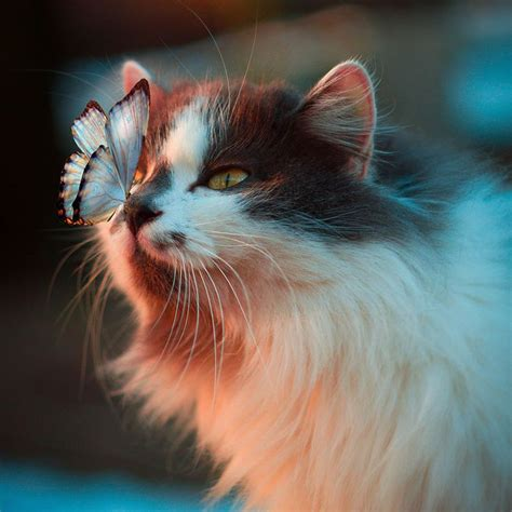
\includegraphics[scale = 0.325]{../Images/Cat/Cat.png}
        \caption{Immagine di un gatto a colori.}
    \end{subfigure}
    \hspace{10pt}
    \begin{subfigure}[b]{0.425\textwidth}
        \centering
        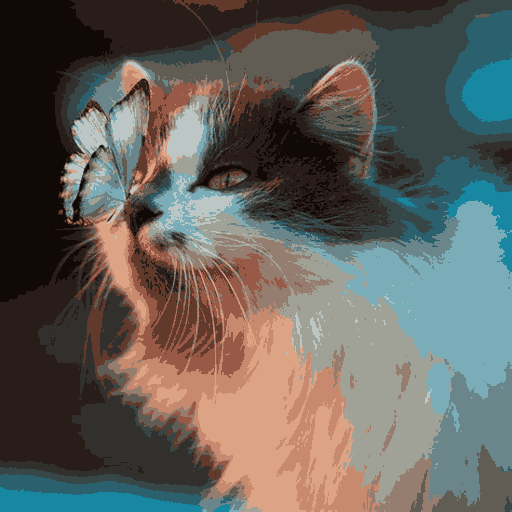
\includegraphics[scale = 0.325]{../Images/Cat/Cat_16.png}
        \caption{Quantizzazione di \emph{Figura \ref{fig:5.3}.a}.}
    \end{subfigure}
    \caption{Esempio di quantizzazione di un'immagine a colore.}
    \label{fig:5.3}
\end{figure}
\end{document}